\section{Foreign Function Interface}
\label{ffi}

In the attempt to have a performant scripting language (luajit) in oure case
with a performant language (C) we need a way for the two to communicate.
For our specific usecase we have the informal line set as ``Smart but slow lua,
and fast but dumb C''.
To achieve this we require a foriegn function interface (ffi) to allow lua to
inform C of what to do.
We compare many ffi implementations, namely:
\begin{itemize}
  \item {\bf Lua C API}: Lua comes with a default Lua C API. Using this method
    requires modification to the C code, but from a Lua perspective the C
    library seems like just another Lua module.
  \item {\bf luaFFI}: The library provides the ability to use the same ffi as
    luajit and requires not modification to the C libraries included.
  \item {\bf dyncall}: Dyncall\cite{dyncall} Is a generic ffi library that has
    bindings to many other languages and enables us to call C functions.  
\end{itemize}

\subsection{What and how to measure}
\begin{figure}[h]
\caption{Measuring FFI performance}
\centering
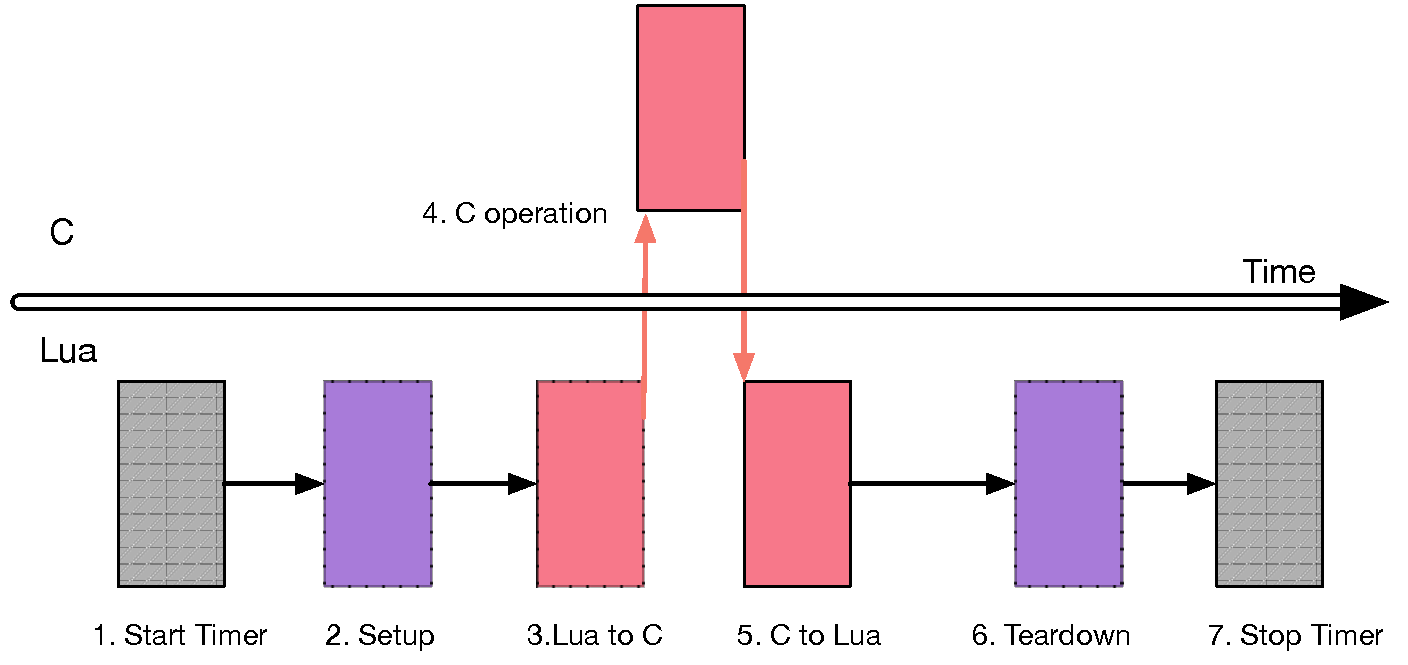
\includegraphics{figs/luac_time.pdf}
\label{ffi_fig}
\end{figure} 

The FFI library consists of mainly three parts. 
The steps involved are a. load the libraries, b. finding the function, and c. executing the found function.
Step a. is not considered by us because this is more of a startup cost, and does not impact the true execution of the ffi modlue selected
 b. and c. on the otherhand are overheads spent int every execution and hence part of our measurement (steps 3, 4, and 5 in Figure~\ref{ffi_fig}).
We would like to keep the c functions essentially no-ops as we are interested in the finding time and the transit time for C to Lua and vice versa.
By performing no-ops we risk thejust in time(JIT) compiler optimizing out that Lua to C code path entirely..
Lastly measuring the start and end times of the test also introduce a point of uncertainity. To minimize this, we measure the time taken by $1$ million transitions between the Lua and C code, where the results of the code is being accumulated and printed at the end of the process.
We present our results in Table~\ref{ffi_bench}. Note that the results are presented as speedup factors instead of absolute numbers (the devision of the absolute number by the baseline). The baseline is se to {\bf lua + luaFFI}.

\begin{tabular}{|l|l|l|l|l|l|l} \hline \hline
\label{ffi_bench}
lua + Lua C API & Luajit + Lua C API & lua + luaffi & luajit & lua + dyncall & luajit + dyncall \\
1.85 & 4.35 & 1.00 & 52.08 & 0.47 & 0.70 \\
\hline
\end{tabular}
% to rebuild these results go to experimental/dyntest and exec ./setup.sh
Based on Table~\ref{ffi_bench} we picked luajit's native ffi routine as our choice. 
